\setcounter{page}{1}
\begin{center}
    \heiti \zihao{-3}基于机器学习的车位规划\\
    \songti \zihao{-4}孙斓绮\\
    (20启新卓越实验(1)班\quad2020339920012)
\end{center}
\songti \zihao{-4}
\section{引言}
近年来,随着我国经济社会的迅速发展,汽车保有量呈现出持续增长的趋势,为人们的生活提供了更便捷的交通工具。据中国汽车工业协会数据显示,截至2023年前10月,汽车产销同比分别增长8\%和9.1\%,达到2401.6万辆和2396.7万辆,如图\ref{fig:cars_sales}所示。这显著的汽车普及趋势加速了城镇化进程\cite{XXCZ202306017},城市密度的激增\cite{JZXB201004006},同时也带来了城市停车资源不足、交通压力大等问题\cite{CSDQ200708009},特别是在土地资源紧缺的情况下,如何高效利用停车资源成为当前城市发展中的紧迫问题。
\begin{figure}[H]
  \centering
  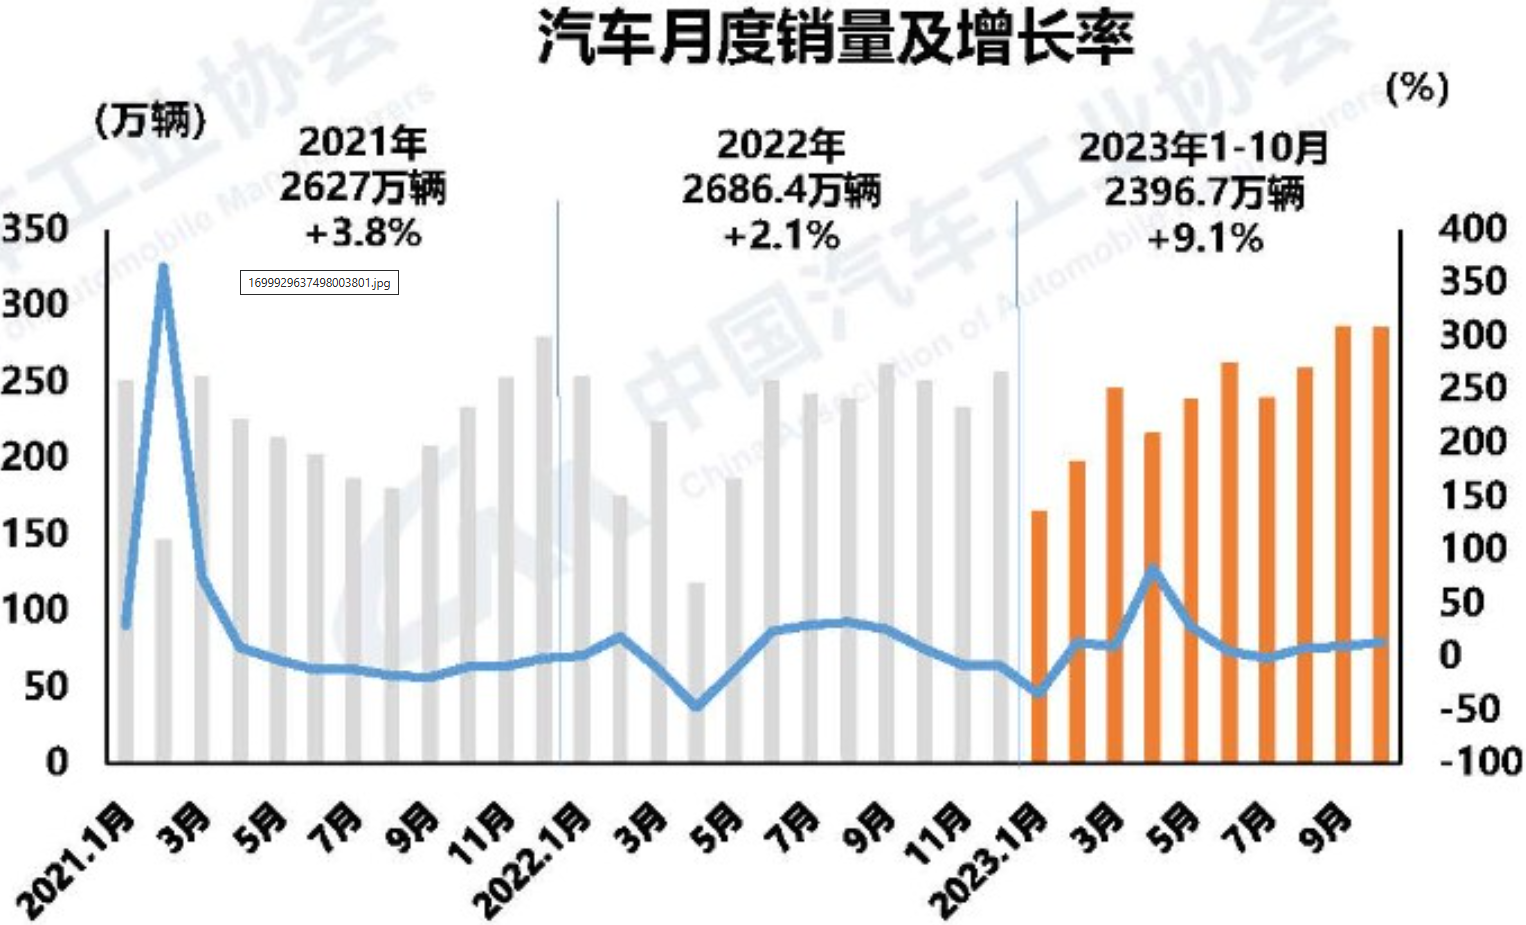
\includegraphics[width=0.7\textwidth]{pictures/汽车月度销量及增长率.png}
  \caption{汽车月度销量及增长率}
  \label{fig:cars_sales}
\end{figure}
为了有效缓解停车难题,地下停车场\cite{JSSD201905002}作为一种解决方案得到了广泛关注。相较于传统的露天停车场,地下停车场在同等土地面积下能够提供更多的停车位\cite{1022811825.nh},同时能够节省城市建设用地,有效缓解地面动静态交通矛盾\cite{CSDQ201807120}。然而,地下停车场设计面临着规范不统一、设计参数复杂\cite{ZGBZ202119043}、结构复杂等一系列问题,尤其是在当前建筑行业的软件发展趋势下,自动化设计成为一种备受期待的解决方案。

本研究旨在借助机器学习的技术,开发一套基于算法的地下车库车位自动化设计系统。通过引入机器学习,缩短设计周期、提高设计效率,同时为设计师提供多样化的设计方案,以适应不同场景的需求。

本文阐述了机器学习在地下车位排布中的应用,对现有的研究工作从地下车库设计和自动化排布等两个方面进行了总结。第 2 节介绍了机器学习的理论知识,总结了机器学习的分类和基础介绍,同时阐明了车位排布这一该场景下的算法选择。第 3 节论述了地下车库设计原理,总结了地下车库布局设计、车位排列方式。第 4 节综述了国内外在从地下车库设计和自动化排布的相关研究工作。最后总结全文并展望了未来研究方向。
\section{机器学习}
机器学习这一术语最早的提出可追溯到上世纪,Arthur Samuel\cite{samuel2000some}等人在其中描述了他使用机器学习来训练计算机玩跳棋的实验,并提出了机器学习是一种使计算机能够进行学习的研究领域。通过多年来诸多学者的研究发现,机器学习致力于研究如何通过让计算机从数据中学习并改善性能,实现对任务的自动化处理。同时,机器学习在多个领域都发挥着关键作用,包括但不限于自然语言处理\cite{young2018recent}、计算机视觉\cite{lecun2015deep}、医疗诊断\cite{esteva2017dermatologist}、金融预测\cite{tsantekidis2017forecasting}等。这些应用领域的研究为机器学习提供了广泛而深刻的实践基础。

一般地,机器学习分为监督学习、无监督学习和强化学习\cite{jordan2015machine},以下便从这三方面来阐述。
\subsection{监督学习}
监督学习是机器学习中的一种基本学习范式,其核心思想是通过从有标签的训练数据中学习输入和输出之间的映射关系,以便模型能够在面对新的、未见过的输入数据时,做出准确的预测。在监督学习中,每个训练样本都包含了输入数据和对应的期望输出(标签),模型通过学习这些样本,不断调整自身参数以提高性能。监督学习适用于各种任务,如分类、回归等。

在车位规划中,获取大规模标记的停车数据可能会非常昂贵且困难;同时,监督学习不适用于动态环境,若停车环境是动态的,由于它只能学习已知标签的模式,因此可能无法很好地适应变化。
\subsection{无监督学习}
无监督学习也同是机器学习中的一种基本学习范式,其特点是在训练数据中没有明确的标签或输出信息。相比于监督学习,无监督学习的目标通常是通过数据本身的内在结构和模式来进行学习和分析。这种学习方式广泛应用于聚类、降维、关联规则挖掘等任务。在无监督学习中,模型通过对输入数据的统计特性、相似性或分布进行建模,从而揭示数据中的潜在结构。无监督学习的应用场景包括但不限于聚类(如K均值算法)、降维(如主成分分析)、关联规则挖掘(如Apriori算法)等。

在车位规划中,由于无监督学习通常是从数据中找到的模式,而非直接关联到标签或奖励,因此生成的模型可能难以解释;并且,它通常是用于探索性分析,可能无法满足特定的停车规划需求。
\subsection{强化学习}
强化学习是一种专注于通过与环境的交互来学习最优行为策略的机器学习方法。与其他学习方式不同,强化学习的学习者在开始阶段并不知道应该采取哪些行动,而是通过试错的方式不断探索,发现哪些行动能够在特定情境下获得最大的奖励。这种学习方式的独特之处在于,学习者必须通过与环境的动态互动逐步改进其行为策略,以达到最优的决策方案。\cite{sutton2018reinforcement}

强化学习相比于前两种学习方式,适用于智能体与环境交互、学习和改进策略的情境,因此对于车位规划中道路、车位、障碍等的交互而言,它是一种自然的选择;与此同时,强化学习还能够考虑到长期奖励,这一点对于车位规划这样的任务来说,模型可以学到更智能、长远的停车策略;还有一点则是,强化学习在适应动态环境方面表现良好,可以通过不断与环境交互来优化策略。

在强化学习中,若要处理复杂的高阶数据\cite{arulkumaran2017deep},通常需要借助深度神经网络作为强大的工具。首次引入深度卷积神经网络到强化学习中的工作由Mnih等人完成\cite{mnih2013playing},他们成功地在Atari 2600游戏上实现了超越人类水平的表现。这种深度神经网络的引入极大地拓展了强化学习的应用领域,使其能够更有效地处理包含丰富信息和复杂特征的数据。
\section{地下车库设计}
\subsection{地下车库布局设计}
鉴于地下建筑通常具有复杂性,设计地下车库时必须注重用户体验。为了创建一个既经济高效又方便安全的地下车库,可以通过增加车位数量、提高通达性以及加强安全性等方面进行优化。因此,在车库的设计布局过程中,需要全面考虑以下几个方面:
\subsubsection{车位数量}
由于地下车库的总面积有限,为了实现更高的经济效益,必须在受限的空间内划分更多的车位。这可以通过增加车库的层数\cite{NMKJ201520021}以及调整车位的排布方式来实现。在进行布局时,需要综合考虑车位的大小、方向、间距以及道路宽度等因素,以最大化地下车库的容纳车位数量。这样的设计优化不仅能够提高车库的利用率,还能够使车库更加经济高效。
\subsubsection{出入口}
对于不同规模的地下车库,出入口的设置至关重要。具体而言,对于车位数小于100的中小型车库,至少需要设置1个出入口;对于车位数不超过1000的中大型车库,至少需要设置2个出入口;而对于车位数超过1000的特大型车库,则需要至少设置3个出入口\cite{CZJS202301011}。

为了提高便捷度,出入口的设置需要充分考虑外部交通状况,并在内部留出足够的通行空间。这样的设计可以有效提升车库的进出效率,使车主在使用车库时能够更加便利和舒适。因此,出入口的科学设置是整个地下车库设计中的重要环节,需要在规模和便捷性之间取得合适的平衡。
\subsubsection{车位轮廓及柱网}
在地下车库中,车位的设计尺寸通常按照小型车为标准,轮廓尺寸为4800mm$\times$1800mm,而实际车位的大小设置为5300mm$\times$2400mm\cite{SCSA201905095, FJJC201712012, CZJS202301011, SCSA202308036}。此外,承重柱的尺寸约为600mm$\times$600mm\cite{FJJC201712012}。

承重柱的设计对于地下车库的安全性和稳定性至关重要。太多的承重柱可能会浪费空间,而太少则难以保证车库的安全性。

为了优化承重柱的设置,可以根据不同柱网规模划分为大、中、小柱网。其中,柱网越大,车库的利用率越高。首选的柱网设计大小为7800mm$\times$8100mm,中型柱网为7800mm$\times$(5000mm$\sim$6100mm),小型柱网为5300mm$\times$(5000mm$\sim$6100mm)\cite{SCSA202308036}。

因此,在规划和设计地下车库时,需要充分考虑车位和承重柱之间的关系,以达到最佳的空间利用和安全性。
\subsubsection{安全性}
安全性方面需要特别关注排水和防火分区设置等问题。在地下车库使用过程中,常常会遇到渗水或积水等问题,而地下与地上建筑之间的关系需要一体化规划和设计。为了防止渗漏问题的发生,必须深入了解地质环境,合理确定地下空间入口与地上的关联性,并通过采取有效措施以达到节能的目的。\cite{YNJC202308018}

另一方面,地下车库的防火分区设计至关重要,以确保设计合理且符合规范。在防火分区设计过程中,需特别关注防火卷帘门的选择。然而,并非每个地下车库都适合使用防火卷帘门。对于某些特殊结构的地下车库,折叠式速降车库门可能更为适用,因为它在防火、防风、防盗等方面能够发挥理想效果。\cite{GXKE202312020}

因此,在地下车库的规划和设计中,需要综合考虑排水、防火分区设置以及防火设备的选择,这是确保地下车库安全性的关键步骤。这样的设计不仅能够有效解决渗水问题,还能够提高车库的整体安全性和防护性。
\subsection{车位排列方式}
为了车位美观、设计灵活,需引入车位模块的概念\cite{1022674189.nh},其中只可放置一种类型的车位。根据规范\cite{ZGBZ202119043}可将模块分为五类,分别为水平、30\textdegree、45\textdegree、60\textdegree、垂直等,具体如图\ref{fig:parking_module}所示。
\begin{figure}[htbp]
  \centering
  \subfloat[垂直车位模块] 
  {
      \label{fig:90_parking_module}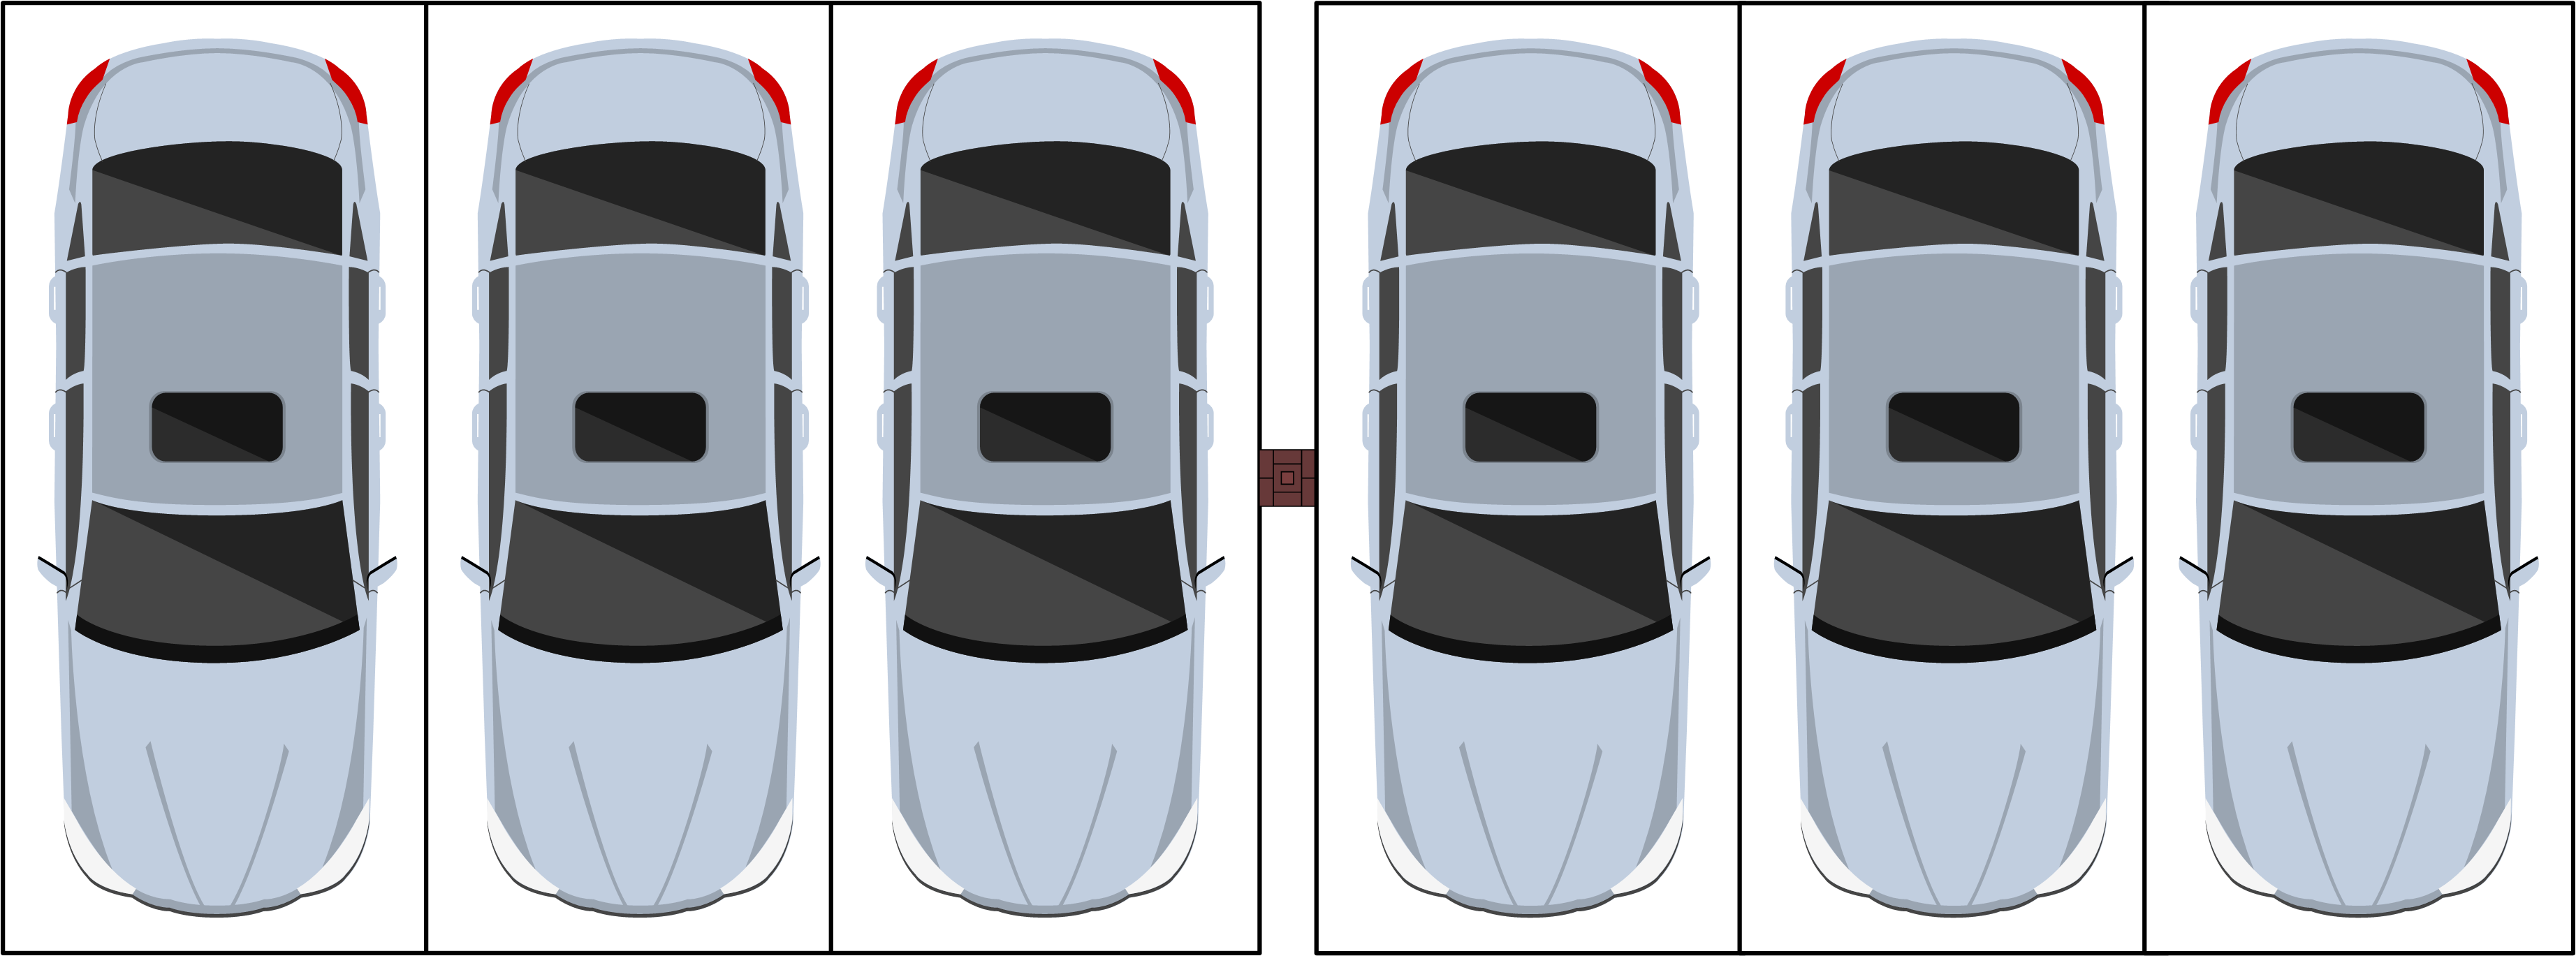
\includegraphics[width=0.4\textwidth]{pictures/车位排列/90.png}
  }\quad
  \subfloat[60\textdegree 车位模块]
  {
      \label{fig:60_parking_module}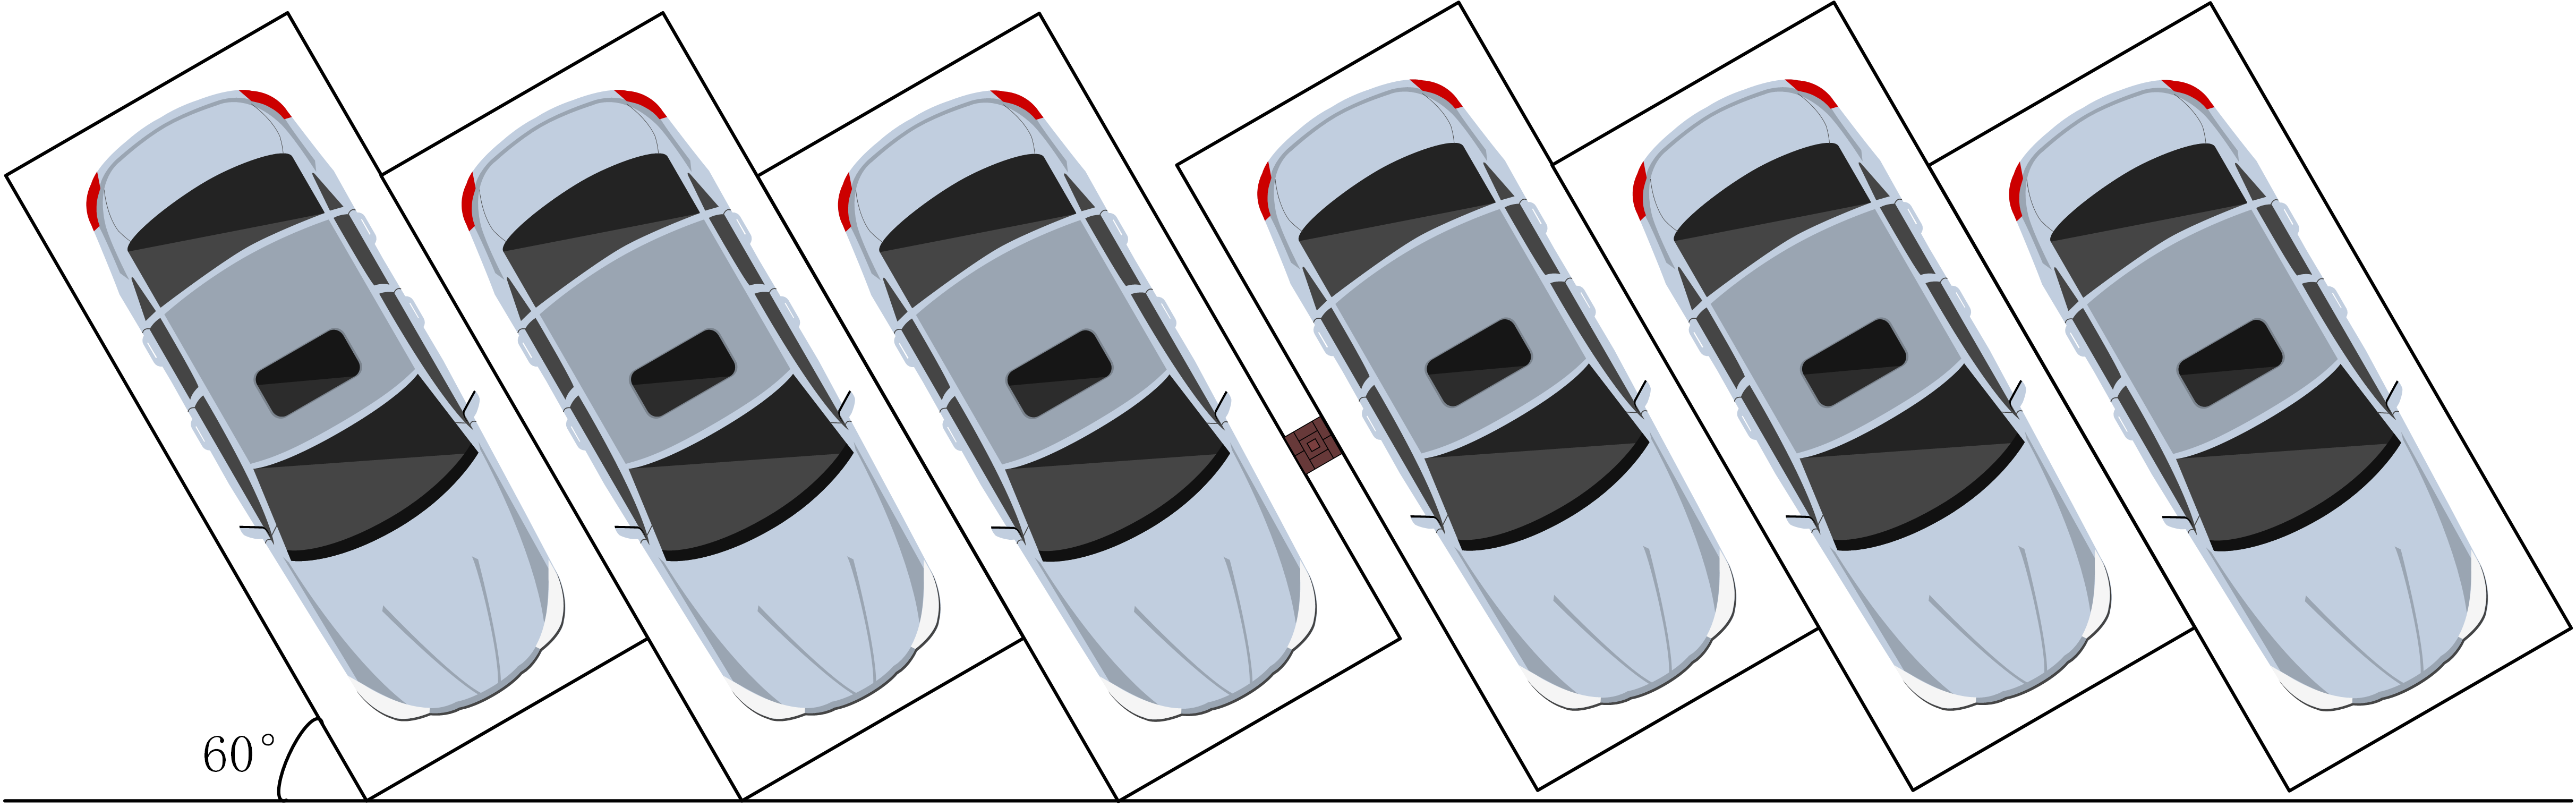
\includegraphics[width=0.4\textwidth]{pictures/车位排列/60.png}
  }\\
  \subfloat[45\textdegree 车位模块]
  {
      \label{fig:45_parking_module}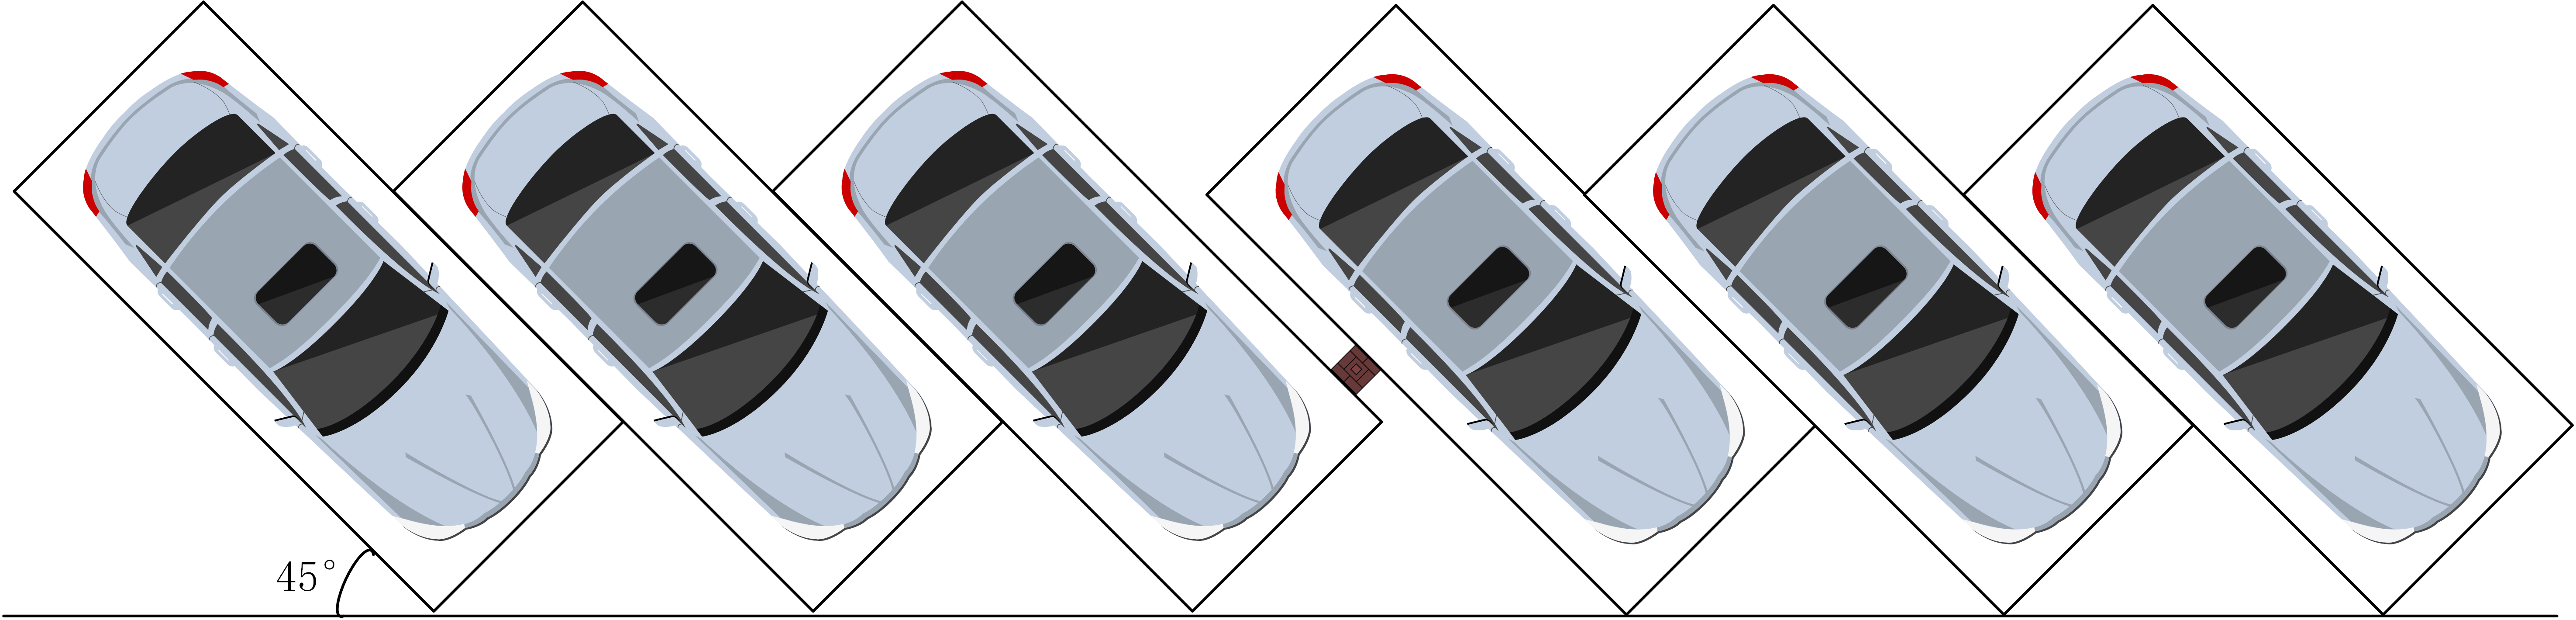
\includegraphics[width=0.4\textwidth]{pictures/车位排列/45.png}
  }\quad
  \subfloat[30\textdegree 车位模块]
  {
      \label{fig:30_parking_module}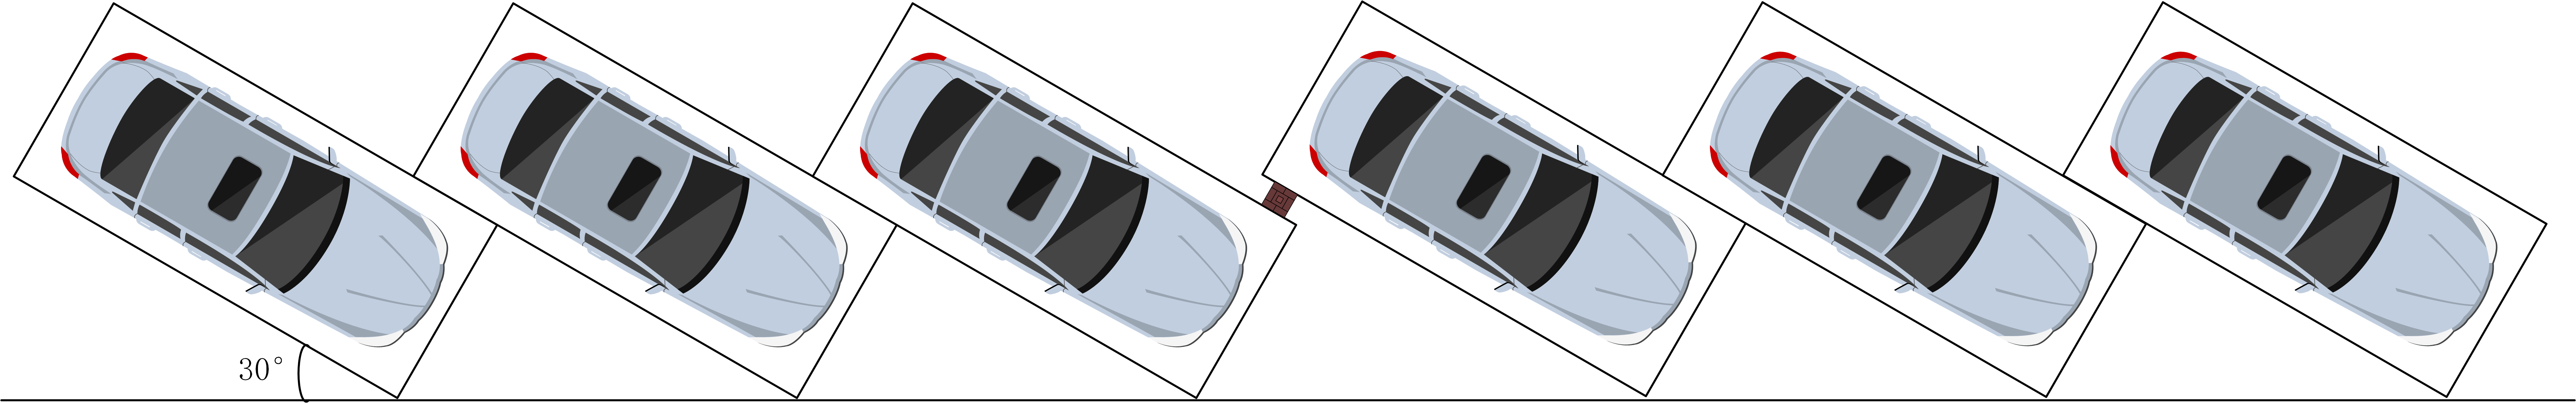
\includegraphics[width=0.4\textwidth]{pictures/车位排列/30.png}
  }\\
  \subfloat[水平车位模块]
  {
      \label{fig:0_parking_module}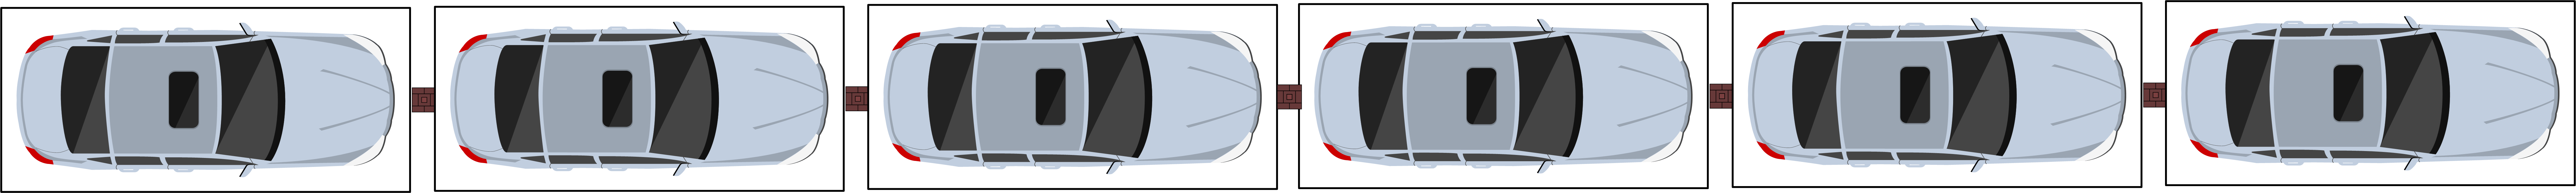
\includegraphics[width=0.8\textwidth]{pictures/车位排列/0.png}
  }
  \caption{5种不同车位模块类型的图示}
  \label{fig:parking_module}
\end{figure}
通过对比,我们可以观察到,随着角度的增大,车位模块的宽度相应减小,这意味着在相同宽度条件下,地块可容纳的车位数量减少。需要注意的是,除了水平和垂直模块外,其他几种角度可能导致较大的空间浪费。与此同时,30\textdegree、60\textdegree、90\textdegree 这三种角度的设计更加符合出行的便利性。

因此在选择排列角度时,需根据实际情况考虑,并综合考虑车位数量、空间利用率、进出便捷度、道路宽度等方面。
\section{国内外研究现状}
\subsection{地下车位布局设计的研究}
国内外专家均对车位布局有一定的研究,该部分也可为自动化排布提供必要参数和理论知识。

Chodash I L\cite{chodash1986relative}等人提出,在67\%的案例中,90度停车对于长度大于100英尺的矩形停车场具有最有效的布局,尽管如此,由于90度停车存在一些固有的缺点,因此并不是在所有情况下都建议采用这一停车角度。Chung S\cite{chen1988optimum}等人通过Ricker方程的计算发现,相较于90\textdegree,70\textdegree 被认为是最佳停车角度,同时,该角度在停车操控性和安全性方面都取得了良好的结果Yousif\cite{yousif2000comparison}等人使用视频技术,研究发现45\textdegree 停车的平均接受间隙高于水平停车。Box\cite{box2002angle}等人证实,水平停车更适合于边缘排布,不仅提升了安全性,而且减少了对交通流量的干扰。Abdelfatah\cite{abdelfatah2014parking}等人则根据三种不同的车位和车道组合,充分利用停车场空间。

相较于国外,国内的发展较晚,但随着汽车的普及,专家逐渐将目光转移到了地下车库的设计上。

Zeng\cite{zeng2009research}等人通过综合考虑路网密度、车辆容量比、车辆出行目的、停车结构、建筑吸收密度以及车辆停车特点等多个因素,提出了一种计算停车需求系数的公式。这篇论文中的相关指标为停车场设计提供了有益的参考。高新涛\cite{HNKJ201518025}采用了平行式、垂直式和斜列式三种停车位布局方式,以实现最大化停车位数量的目标,同时保证了模型的有效性。谷锦彪\cite{1017056100.nh}通过分析停车行为特性,利用ROC判别模型计算不同角度时,推荐的车位尺寸,还得出45\textdegree 比60\textdegree 更为合理的结论。Liu J\cite{liu2021parking}提出了一种基于模糊综合评价方法的车位预留模型,适用于车位不足的情况。

这些国内外研究为停车场设计在停车角度、间隙与车位预留状况等方面均提供了丰富的理论和实践经验。
\subsection{车位自动化排布研究}
1981年时,Fowler\cite{fowler1981optimal}证明了不带约束的排样问题是NP完全问题,而地下车位排布可被看作是带空洞的二维排布问题。
针对类似矩阵的地下车库,Birgin\cite{birgin2006method, birgin2006orthogonal}提出了“哨兵“和非线性规划的通用解法,在任意凸区域内都有较好的效果;后续在2010年又得到了改进\cite{birgin2010orthogonal},使得矩形件可旋转。随着机器学习算法的普及,专家逐渐在将排布与机器学习算法结合。Xu YC\cite{xu2007particle, xu2010genetic}引入了粒子群算法和搜索最优定位顺序的遗传算法均优化了性能。L{\'o}pez\cite{lopez2018packing}等人使用了一种混合整数非线性规划的模型,来解决圆形容器中的问题。马莹\cite{JSGG201820015}等人提出了自适应量子遗传算法,旨在优化问题求解,并提高材料利用率。

但实际上来看,车位排布相比于矩形排样多了一些有关车道、车位、障碍物等的限制条件。Hasbiyati\cite{hasbiyati2019parking}等人提出了一种平行四边形形式的停车场的排布,其中平行四边形看作为两个三角形的组合来进行计算。Huang\cite{huang2020general}等人研究了基于贪婪算法的单双边停车通道布局选择。Timpner\cite{timpner2015k}等人提出了自动代客泊车的车位优化,Banzhaf\cite{banzhaf2017high}等人基于前面的优化提出了混合整数规划模型,Nourinejad\cite{nourinejad2018designing}等人,基于排队路构建了混合整数模型,设计了一种启发式算法,利用Benders进行分解。Syahrini\cite{syahrini2018mathematical}等人建立了三角形停车场的优化模型,并尝试在等腰和等边三角形中进行尝试。

同时,随着自动停车或是自动驾驶车辆的出现,车库也将迎来新的革新。Ferreira\cite{ferreira2014self}等人,利用半自动和全自动驾驶技术,以协作方式为进出停车场的汽车创造空间,这种方式极大地提高了土地利用率,也减少了出入时间,但对汽车类型要求严苛。Siddique\cite{siddique2021puzzle}等人通过小型停车场的最佳排布结果,用启发式算法生成大型停车场的解。

由于大部分的车库轮廓并非规则,且通常有不规则障碍排布,同时自动车辆未普及。针对此类问题,徐涵喆\cite{1020726891.nh}一种基于遗传算法的外圈车位排布的启发式算法,主要提供了针对外圈的处理方法。黄逸彬等人\cite{BJYD202004002}开发了基于图形分割的粒子群优化算法。冯嘉宇\cite{1022674189.nh}提出了内外圈分离算法,内圈使用像素分割算法,外圈则是使用遗传算法,从而充分利用空旷面积。但这些研究都无法充分利用车位与边界的区域,且在障碍物较多的情况下效果较差。

对于强化学习技术在地库排布的应用,余光鑫\cite{1020332216.nh}提出了一种基于强化学习的地下车库生成式设计方法,主要针对规则边缘的场地,边铺设地面边放置车位。团队使用简单的网络结构以及进化策略,来淘汰奖励少的个体。该方法虽提高了算法的决策力和准确度,但仍存在时间开销大、对于不规则轮廓地库的学习难度大等问题。王潇霆\cite{1023719817.nh}也是通过强化学习,但他改变了每轮结束再集奖励的方式,而是每走一步均有奖励,但奖励并非连续函数,可解释性较差。对于不同区域的放置方式,主要借助于车位模块,非边界可通过区域分割,边界则是运用组合式车位放置的方法进行,与冯嘉宇不同,他的障碍周边没有道路,因此不可直接在内部进行排位,需根据其周围情况进行分类讨论。

这些国内外研究表示,开始时专家们采用非线性规划、粒子群算法、遗传算法等方法进行优化。随着机器学习的应用,排布问题与机器学习相结合。而新技术如半自动和全自动驾驶的出现,也推动车库设计往提高土地利用率的方向进行创新。同时,强化学习技术引入地下车库设计,尽管存在一些挑战,如时间开销和对不规则轮廓的学习难度,但仍具有广阔的应用前景。
\section{总结与展望}
本文综述了地下车库设计与研究的现状,以及车位自动化排布的相关研究。在地下车库设计方面,专家们通过对停车角度、车位模块、停车需求系数等多个因素的考虑,提出了各种布局方案和优化方法,为停车场设计提供了丰富的理论和实践经验。在车位自动化排布方面,研究者们采用了多种算法,包括哨兵算法、粒子群算法、遗传算法等,以解决地下车库的车位排布问题,提高了土地利用率和停车效率。

目前的研究还存在一些问题和挑战。对于不规则轮廓的地下车库和空洞内地车位排布,现有算法的效果有限,难以充分利用车位与边界的区域以及障碍群里的空间。强化学习技术在地库排布的应用仍然面临学习难度大、时间开销大等问题。因此,未来的研究可以进一步深化对不规则轮廓地下车库的排布算法的研究,提高算法的适应性和智能化水平。

此外,随着自动驾驶技术的发展,未来地下车库的设计可能会更加注重与自动驾驶车辆的协同,以提高停车场的智能化水平。研究者可以探索更先进的强化学习算法,结合实际场景中的障碍物、车流等因素,进一步提高自动排布的效果。